\chapter{Hardware-Anpassungen}
In diesem Kapitel wird darauf eingegangen, welche Hardware-Anpassungen im Prozessor vorgenommen wurden, um in den Algorithmen eine Verbesserung der Verlustleistung zu ermöglichen.
\section{Pipelinestufe für Adressports}
Da der verwendete Prozessor eine Adress-Isolation (siehe Kapitel \ref{subsec:add_iso}) einsetzt, sollten die Adressen so lange an einem Port anliegen, bis diese geändert werden.
Die für die Schreib- und Lesezugriffe verwendeten Adressen werden jeweils zwischen den Takten von dem Adress-Decoder berechnet und an die benötigten Ports angelegt. Dadurch ist gewährleistet, dass diese mit der steigenden Taktflanke übernommen werden können. Die Auswahl der Ports wird über Enable-Signale geregelt. Im Fall dieser Architektur treten Glitches auf, die auf Grund der unterschiedlichen Berechnungszeiten der Kombinatorik verursacht werden. In Schaubild \ref{fig:glitches} wird dieses Verhalten veranschaulicht. Hier ist zu erkennen, dass das Enable-Signal schaltet, bevor die neue Adresse angelegt wird. Dadurch wird ein Glitch in den Adressleitungen verursacht. Im Schaubild werden die Registerport-Adressen angezeigt, die nicht angesprochen werden sollen, da dort die Glitches am deutlichsten erkennbar sind. Dieses Szenario tritt nur auf, wenn ein Wechsel in den Enable-Signalen stattfindet und sich somit die Herkunft der Adressen geändert hat.
% Werden beispielsweise zwei Instruktionen verwendet die beide an Register-File 1 schreiben, so werden die entsprechenden Adressen an die Ports 0 und 1 angelegt. Sobald diese zu Verfügung stehen, werden diese von den Enable-Signalen freigegeben.\\

\begin{figure}[H] 
	\centering
	\includesvg[width=0.70\textwidth]{glitches}
	\caption{Glitches Write-Adress}
	\label{fig:glitches}
\end{figure}


% Dies liegt daran, dass die benötigten Enable-Signale aufwendig berechnet werden müssen und dies eine kurze Verzögerung nach sich zieht
Das beschriebene Problem verursacht eine Erhöhung der Schaltaktivität auf den Adressleitungen. Dadurch steigt die Verlustleistung in den Testfällen an den einzelnen Adress-Ports um teilweise bis zu 49,44\%.
Um diesem Effekt entgegenzuwirken, wurde eine weitere Pipeline-Stufe eingebaut. Diese verzögert die Adressen so, dass keine Glitches an die Register-Ports weitergeleitet werden (siehe Abbildung \ref{fig:glitches_pipeline}). Der zusätzliche Energieverbrauch der Pipeline-Register wird an dieser Stelle nicht weiter untersucht, da der Anstieg der Verlustleistung in den zu vergleichenden Algorithmen identisch ist.

\begin{figure}[H] 
	\centering
	\includesvg[width=\textwidth]{glitches_pipeline}
	\caption{Pipelinestufe gegen Glitches}
	\label{fig:glitches_pipeline}
\end{figure}

%\begin{figure}[!ht]
%	\centering                  % zentrierte Ausrichtung
%	\def\svgwidth{200pt}    % die Bildbreite festgelegt
%	%\includegraphics{test1.pdf}
%	\input{fig/glitches_pipeline.pdf_tex} %hier ist meine text Datei
%	\caption{test}    % Bildunterschrift
%	\label{fig:test}          % Label für Verweise
%\end{figure}

Es besteht jedoch eine Möglichkeit, die Pipeline-Stufen zu vermeiden.
Da der Prozessor für ein ASIC entwickelt wird, können die Glitches durch den Einsatz von Buffern behoben werden. Hierzu müssen lediglich die Enable-Signale mittels im ASIC implementierter Buffer verzögert werden. Dieser kann beispielsweise durch das Einbauen zwei hintereinander geschalteter Inverter realisiert werden. Dabei ergibt sich die Verzögerung aus der Summe der Gatterlaufzeiten. Die Anzahl der Inverter-Gatter muss dann an den Versatz von Adress- und Enable-Signal angepasst werden.

\section{Neuberechnung der Immediate-Adressen und Offset-Werte}
Die im Implementierungsteil erläuterten Änderungen sollten keinen Einfluss auf die Daten der auszuführenden Algorithmen haben. Beim Vergleich der Implementierungen ist jedoch eine Abhängigkeit der Daten aufgetaucht.\\
Die Decoding-Stage berechnet, unabhängig von den angelegt Instruktionen, aus jeder Adresse eine Immediate-Adresse und leitet diese an die Exekution-Stage weiter. Dort werden Source-Adressen für kurze Zeit als Immediate-Adressen interpretiert und verursachen dadurch Schaltaktivitäten an den Daten-Leitungen. Diese Veränderung der Daten ist nicht erwünscht und wurde aus diesem Grund mittels Anpassung der Hardware entfernt. Um das beschriebene Phänomen zu beheben, wird eine Neuberechnung der Immediate-Adresse nur dann vorgenommen, wenn es sich bei der angelegten Instruktion auch um eine Immediate-Instruktion handelt.
Mittels dieser Veränderung ist die Verlustleistung nun nicht mehr von den Daten abhängig.

Die selbe Vorgehensweise wurde bei der Neuberechnung der Offset-Werte angewandt, so dass auch hier keine ungewollten Schaltaktivitäten auftauchen.



\chapter{Evaluation}
\label{chap:evaluation} 
Damit die implementieren Algorithmen hinsichtlich der Verlustleistungsoptimierung verifiziert werden können, werden diese auf Gatterebene in einer 40 nm ASIC-Technologie getestet. Da die Verlustleistung nicht zur Laufzeit des Codes bestimmt werden kann, muss eine Verlustleistungssimulation nach der Ausführung des Codes stattfinden. Die Vorgehensweise um von einem Assemblerprogramm zu einem Power-Report zu gelangen, ist in Schaubild \ref{fig:flow_power_analyse} abgebildet.

\begin{scriptsize}
	\begin{figure}[htbp] 
		\centering
		\includesvg[width=0.50\textwidth]{evalution_flow}
		\caption{Power-Analyse Ablaufdiagramm}
		\label{fig:flow_power_analyse}
	\end{figure}
\end{scriptsize}

Vorerst wird das gewünschte Assemblerprogramm zusammen mit der Prozessorkonfiguration in den Scheduler geladen. Hierbei muss unter anderem angegeben werden, mit welchen Takten der Prozessor taktet. Außerdem muss dem Scheduler die Variante der zu verwendenden Register-Allokation (Tabelle \ref{tab:algo_conifg}, Kapitel \ref{chap:register_orga}) übergeben werden. Nach erfolgreichem Kompilieren des Codes steht die Binary-Datei und der geschedulte Code zur Verfügung. Im Anschluss an diesen Prozess wird die Leistungsanalyse durchgeführt. Hierzu wird die Netzliste des Prozessors und die Binary-Datei benötigt. Das Tool \glqq Prime Time Suite\grqq{ }von Synopsys analysiert alle Schaltaktivitäten im Prozessor und gibt anschließend eine detaillierte Übersicht über die Leistungsaufnahme des Prozessors aus.\\
Hierbei wird die Leistung in Internal-, Switching- und Leakage-Leistung aufgeteilt. Die Leakage-Leistung ist so definiert, dass alle Zeiten in der eine Zelle nicht benutzt wird oder ihren Zustand nicht ändert, aufsummiert werden und mit den jeweiligen Transistor-Konfigurationen verrechnet werden. Dabei gibt es zwei verschiedene Ströme, die die Verlustleistung verursachen, der Gate-Leakage-Strom $I_{gl}$ und der Source-Drain-Strom $I_{lk}$ (siehe Abbildung \ref{fig:prime_time_power}). Bei der Leakage-Leistung handelt es sich somit um eine statische Verlustleistung. Hingegen sind Internal- und Switching-Leistung dynamische Verlustleistungen, die von den Schaltvorgängen beeinflusst werden. Die Internal-Leistung inkludiert alle Leistungen, die in einer Zelle durch das Laden/Entladen von Kapazitäten mit dem Strom $I_{SW}$ und auf Grund der Kurzschluss-Ströme $I_{SC}$ verursacht werden. Dagegen sind in der Switching-Leistung die Verlustleistungen berücksichtigt, die durch das Laden von externen Lastkapazitäten verursacht werden.\cite{primeTime2016}
\begin{figure}[H] 
	\centering
	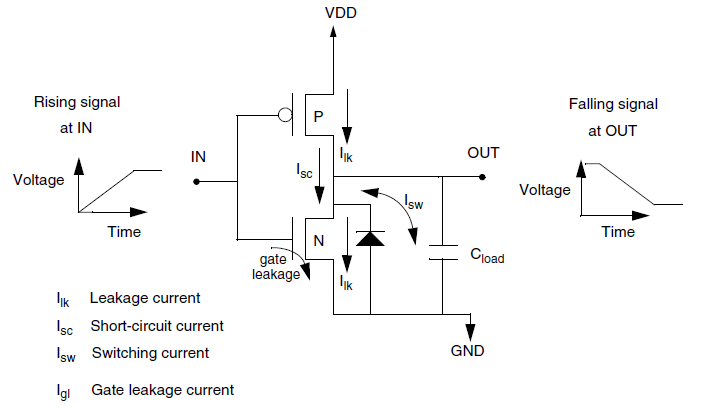
\includegraphics[width=\textwidth]{prime_time_power}
	\caption[Komponenten der Leistungsaufnahme]{Komponenten der Leistungsaufnahme \cite{primeTime2016}}
	\label{fig:prime_time_power}
\end{figure}
Mithilfe dieses Evalutionsablaufes sind die in diesem Kapitel evaluierten Ergebnisse entstanden.
\section{Testprogramme}
Um den Einfluss der Register-Adressen besser verstehen zu können, wurden Assemblerprogramme entwickelt, die den Einfluss von Target-, Source1- und Source2-Registern untersuchen. Hierbei sind die Testfälle nach Komplexität gestaffelt. In den folgenden Kapiteln wird nun auf die Ergebnisse der einzelnen Programme und deren Erkenntnisse eingegangen.
\subsection{Empirische Tests}
\label{cap:empirischeTests}
Um die aufgestellte Annahme, dass sich die Verlustleistung proportional zur Hamming-Distanz verhält, zu bestätigen, wurden zu Beginn Assemblerprogramme entworfen, die nur mit physikalischen bzw. festen Registern arbeiten.
Außerdem wurden vorerst der Best- und Worst-Case untersucht, um das maximale Optimierungspotential zu ermitteln. Das Programm durchläuft dabei alle Möglichkeiten der Adress-Port-Zuweisung. Es testet zum einen die Register-Allokation und die damit verbundene Hamming-Distanz-Berechnung, zum anderen werden alle Einflüsse der Register-Adressierung ermittelt. Da der Prozessor zwei Register-Files mit jeweils zwei Write- und vier Read-Ports aufweist, bestehen für die Target-Register vier und für die Source-Register 16 Möglichkeiten der Portzuweisung (siehe Tabelle \ref{lese-port} sowie \ref{fig::schreib-port}). Dabei sind X2-Operationen ausgenommen. Im Worst-Case werden die Register so adressiert, dass die maximale Hamming-Distanz entsteht. Dabei wechseln die Adressen von Null auf 31, welches der maximalen Hamming-Distanz von Fünf entspricht. Damit keine Einflüsse durch Scheduling oder Daten entstehen, wurden Instruktionen manuell geschedult und den einzelnen Issue-Slots zugewiesen. Somit ist die Anordnung der Assemblerbefehle für jeden Testfall identisch und der Einfluss ist demzufolge entkoppelt. Im Falle der Datenabhängigkeiten werden alle Register mit einer Null initialisiert und im Anschluss nicht verändert. Dadurch werden alle Instruktionen mit den selben Daten ausgeführt.
Für den Fall des Best-Case wird die Adresse nicht verändert und immer von der Adresse Null gelesen, beziehungsweise auf sie geschrieben.
Das Power-Analyse-Tool zeigt nach dem Ausführen des Workflows (Abbildung \ref{fig:flow_power_analyse}) eine Übersicht über die Leistungsaufnahme des Prozessors an. Hierbei wird die Leistung in Internal-, Switching- und Leakage-Leistung aufgeteilt (siehe Abbildung \ref{fig:best_power_hierarchy}).
Diese Leistungen werden hierarchisch nach den einzelnen Prozessor-Modulen aufgeschlüsselt. Die letzte Spalte des Reports zeigt die Aufteilung der Leistungsaufnahme in Prozent. Dabei ist zu erkennen, dass das Register-File (vrf\_inst) mit 65,2\% die größte Leistungsaufnahme im Prozessor aufweist.

\begin{figure}[H] 
	\centering
	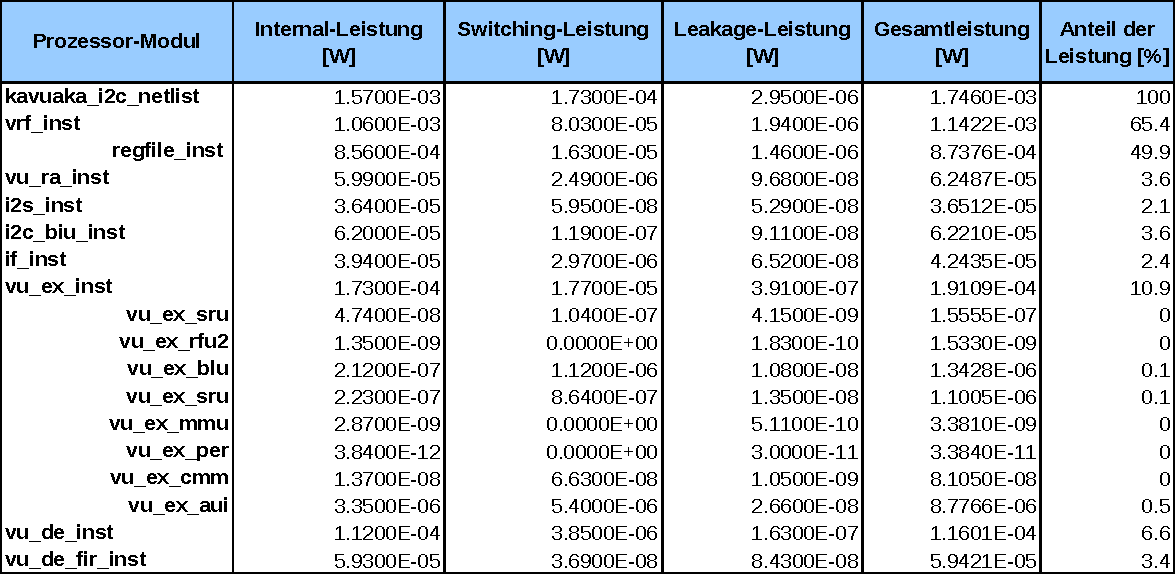
\includegraphics[width=\textwidth]{fig/best_hierarchy_report.pdf}
	\caption{Best-Case hierarchische Leistungsaufnahme}
	\label{fig:best_power_hierarchy}
\end{figure}

Aus beiden ermittelten Reports für den Worst- und Best-Case wurde die Tabelle \ref{fig:best_powersave} erzeugt. Dabei sind die Einträge in Prozent angegeben und zeigen ein deutliches Einsparungspotential. Außerdem sind alle Prozente auf die Gesamtleistung der entsprechenden Spalte bezogen. Das Augenmerk sollte hierbei auf die Switching-Leistung des Register-Files gelegt werden, denn hier wurden die Veränderungen in der Adressierung erzeugt. Dabei ist deutlich zu erkennen, dass eine maximale Einsparung von 18,33\% zu erreichen ist. Dies zeigt deutlich, dass die Adressierung der Register eine Auswirkung auf die Verlustleistung hat. In den anderen Modulen des Prozessors wurden ebenfalls Verbesserungen zu erzielt. Das liegt vor allem daran, dass die Register-Adressen ebenfalls in diesen angelegt sind. Bei der Execution-Stage ist keine Verbesserung erzielt worden, da dort nur die Daten der jeweiligen Instruktion anliegen. Die Verbesserung der internen Leistungsaufnahme kann damit begründet werden, dass die Adressen ebenfalls Einfluss auf die interne dynamische Verlustleistung haben.
Das Resultat der unterschiedlichen Adressierungen ist eine Gesamtverlustleistungseinsparung von 7,87\%.

\begin{figure}[H] 
	\centering
	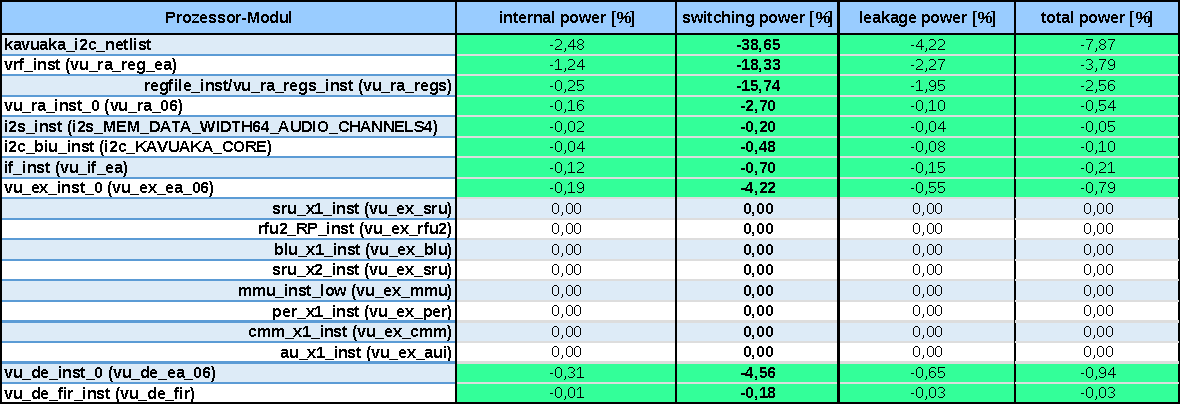
\includegraphics[width=\textwidth]{fig/best_worst_compare.pdf}
	\caption{Einsparungspotential Best-Worst-Case}
	\label{fig:best_powersave}
\end{figure}
\subsection{Synthetische Testprogramme}
Da nun gezeigt wurde, dass ein Zusammenhang zwischen Adressierung und Verlustleistung besteht, wird die Register-Allokation weiter untersucht. Hierzu wurden synthetische Testfälle erstellt, welche mit unterschiedlichen Adressierungen, aber den selben Daten, arbeiten. Dabei wurden vorerst die Register einzeln betrachtet. Um die einzelnen Ergebnisse vergleichen zu können, wurden die Programme so entworfen, dass die Hamming-Distanzen für alle Testfälle identisch ausfallen. Das heißt, die Schaltaktivitäten in den Lese- sowie Schreibports sind identisch und die Leistungen können somit verglichen werden. Ein Beispiel für ein solches Testprogramm, welches den Einfluss der Target-Register testet, ist in Codebeispiel \ref{code:target_switching_test} zu sehen. Um die Source-Register vom Test zu entkoppeln, wurden die Adressen der Register, die nicht untersucht werden sollten, nicht verändert. Dadurch entsteht keinerlei Schaltaktivität in den Adressleitungen. Gestartet wird die Berechnung der Hamming-Distanz immer mit der Adresse 0, da keine Aussage getroffen werden kann, welche Adresse in der letzten SLM zugewiesen wurde.

\begin{algorithm}[H]
	\begin{algorithmic}[1]
		\STATE {:0 \textbf {ADD} V0R2 V0R0 V1R0 \hspace{50pt}:1 \textbf {OR} V0R2 V0R0 V1R0}
		\STATE {:0 \textbf {ADD} V0R0 V0R0 V1R0 \hspace{50pt}:1 \textbf {OR} V1R2 V0R0 V1R0}
		\STATE {:0 \textbf {ADD} V1R0 V0R0 V1R0 \hspace{50pt}:1 \textbf {OR} V0R2 V0R0 V1R0}
		\STATE {:0 \textbf {ADD} V1R2 V0R0 V1R0 \hspace{50pt}:1 \textbf {OR} V1R2 V0R0 V1R0}
		\STATE {:0 \textbf {ADD} V0R0 V0R0 V1R0 \hspace{50pt}:1 \textbf {OR} V0R0 V0R0 V1R0}
		\STATE {:0 \textbf {ADD} V0R2 V0R0 V1R0 \hspace{50pt}:1 \textbf {OR} V1R0 V0R0 V1R0}
		\STATE {:0 \textbf {ADD} V1R2 V0R0 V1R0 \hspace{50pt}:1 \textbf {OR} V0R0 V0R0 V1R0}
		\STATE {:0 \textbf {ADD} V1R0 V0R0 V1R0 \hspace{50pt}:1 \textbf {OR} V1R0 V0R0 V1R0}
		\caption{Codebeispiel Target-Register }
		\label{code:target_switching_test}
	\end{algorithmic}
\end{algorithm}

Dieser Test wurde für die Adressen Zwei, Fünf, 24, 25, 27 und 31 ausgeführt. Außerdem wurden Target, Source 1 und Source 2 getestet. Die untenstehenden Schaubilder (\ref{fig:source0_power}., \ref{fig:source1_power}., \ref{fig:target0_power}. sowie \ref{fig:target1_power}.) zeigen die Schaltleistung der verschiedenen Testfälle. Es ist zu erkennen, dass die Schaltleistungen der Lese- sowie Schreibports linear mit der Hamming-Distanz steigen. Außerdem sind die Graphen der Source-Register nahezu identisch, was impliziert, dass die Adressen in den Lese-Ports die gleiche Verlustleistung verursachen.\\

\begin{figure}[H]
	\centering
	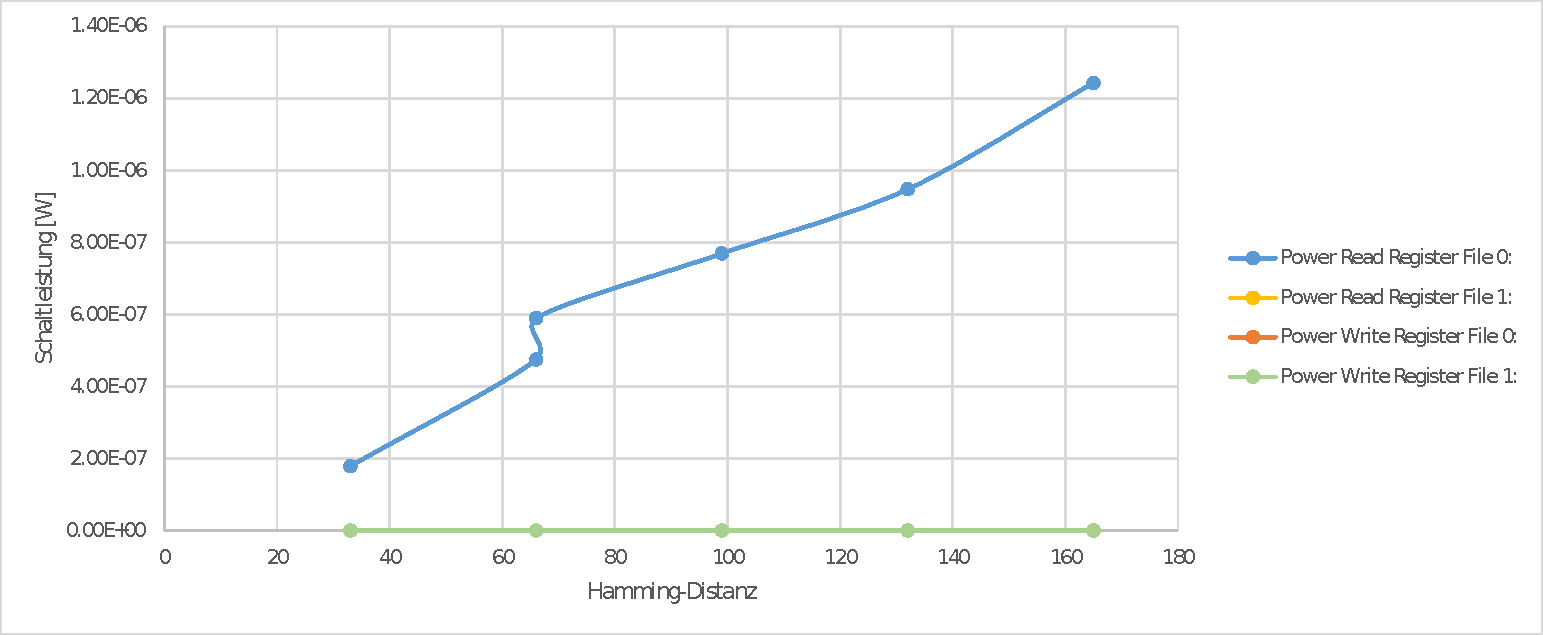
\includegraphics[width=\textwidth]{fig/source1_power.pdf}
	\caption{Schaltleistung Read Register File 0}
	\label{fig:source0_power}
\end{figure}
\begin{figure}[H]
	\centering
	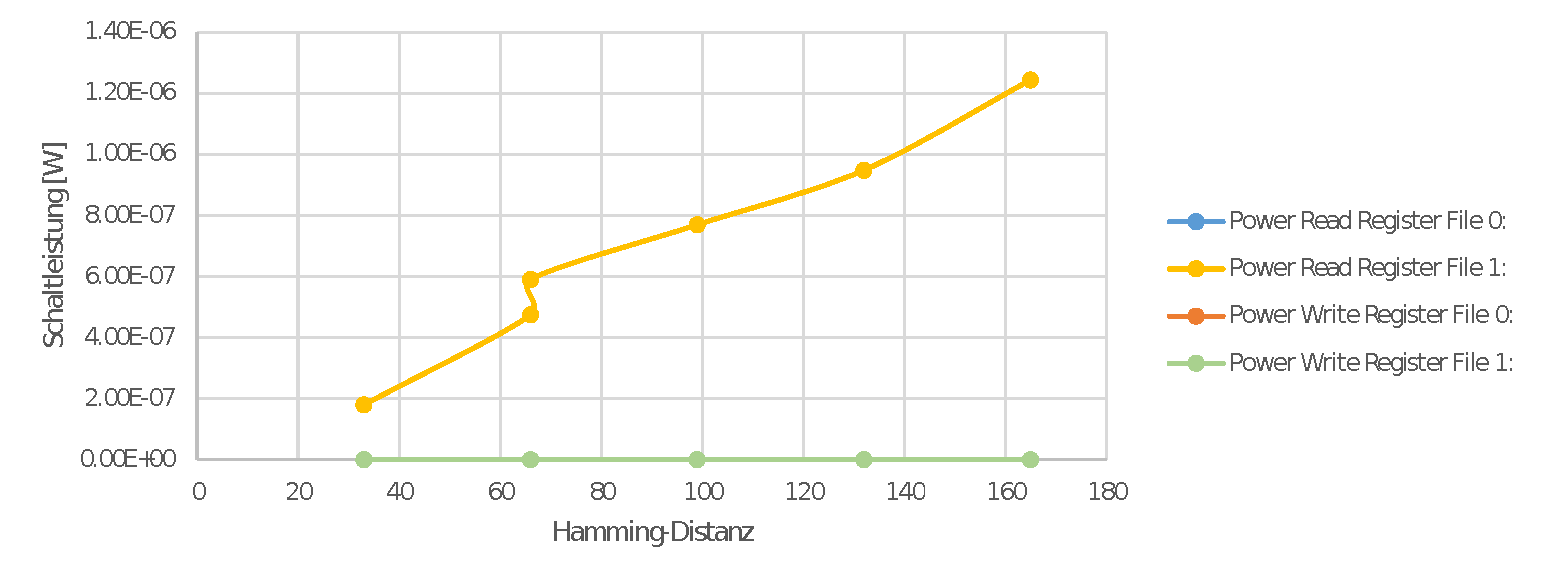
\includegraphics[width=\textwidth]{fig/source2_power.pdf}
	\caption{Schaltleistung Read Register File 1}
	\label{fig:source1_power}
\end{figure}
\begin{figure}[H]
	\centering
	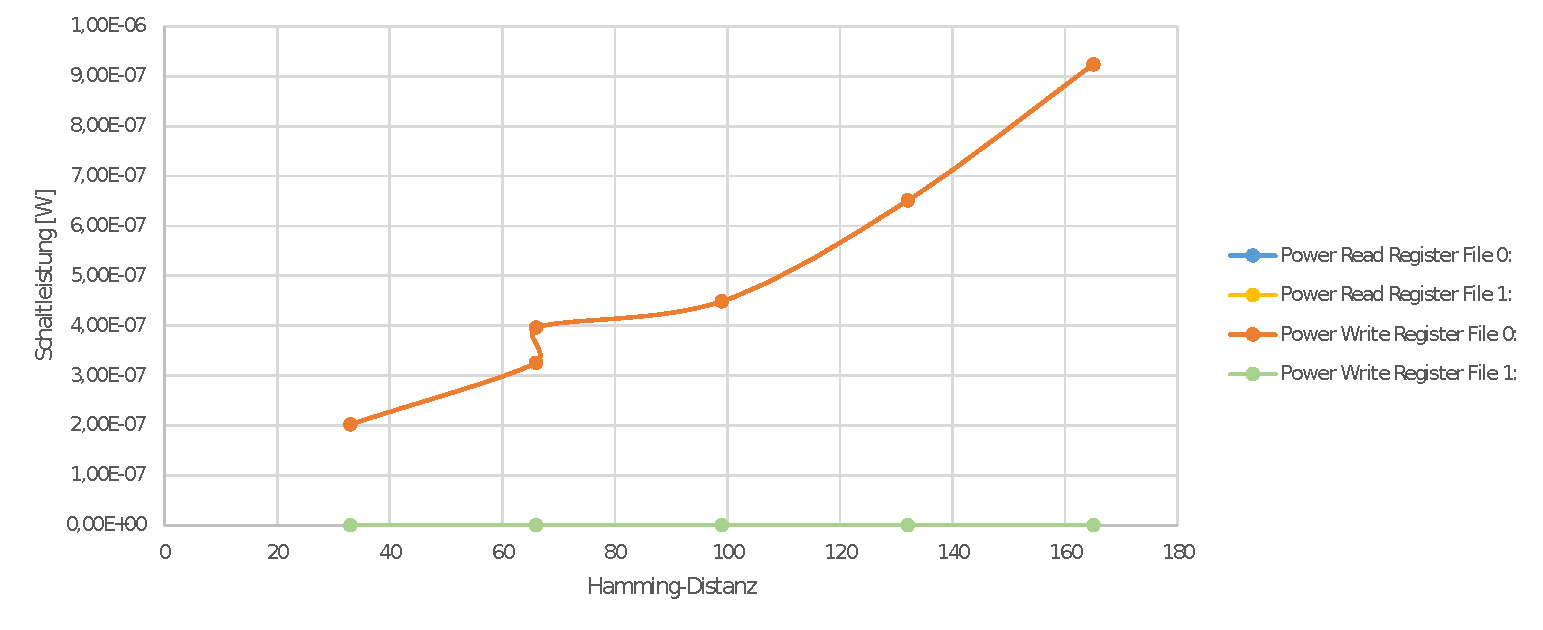
\includegraphics[width=\textwidth]{fig/register_eval_target_port0.pdf}
	\caption{Schaltleistung Write Register File 0}
	\label{fig:target0_power}
\end{figure}
\begin{figure}[H]
	\centering
	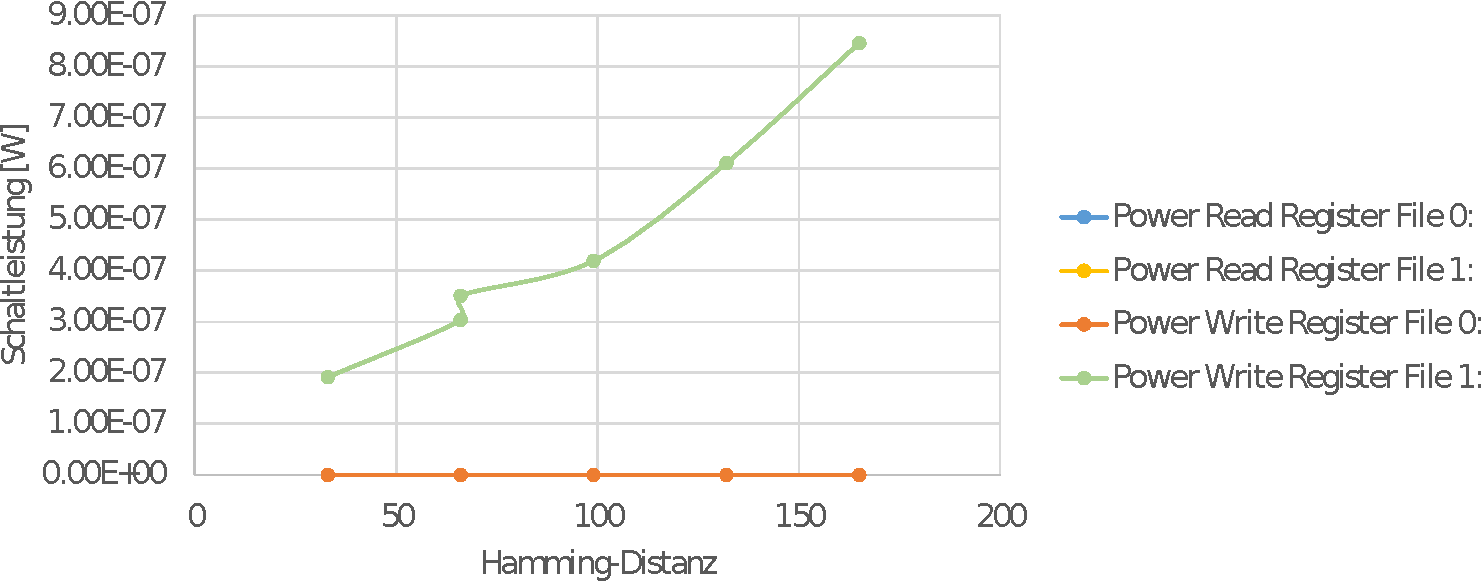
\includegraphics[width=\textwidth]{fig/register_eval_target_port1.pdf}
	\caption{Schaltleistung Write Register File 1}
	\label{fig:target1_power}
\end{figure}

Bei allen vier Graphen ist ein Sprung der Leistung bei einer Hamming-Distanz von 64 auffällig. Dieser Sprung lässt sich dadurch erklären, dass zwar die Hamming-Distanzen der Testfälle mit den Register-Adressen Fünf und 24 identisch sind, aber unterschiedliche Adressleitungen verwendet werden, welche eine größere Lastkapazität aufweisen. Durch die höhere Lastkapazität wird automatisch auch eine größere Leistung benötigt. Dieses Phänomen wird in Kapitel \ref{cap:lastkapa} näher untersucht und erläutert.\\
Nachdem die Register getrennt voneinander betrachtet wurden und sich gezeigt hat, dass die Adressen ungefähr die selben Schaltleistungen in den Ports verursachen, wird das Verhalten beim gemeinsamen Schalten der Source- sowie Target-Register untersucht. Auch hierbei werden die Tests mit den selben Hamming-Distanzen für Lese- und Schreib-Ports ausgeführt. Das Schaubild \ref{fig:source_target_power} zeigt auch hier, dass ein linearer Verlauf erkennbar ist.

\begin{figure}[H]
	\centering
	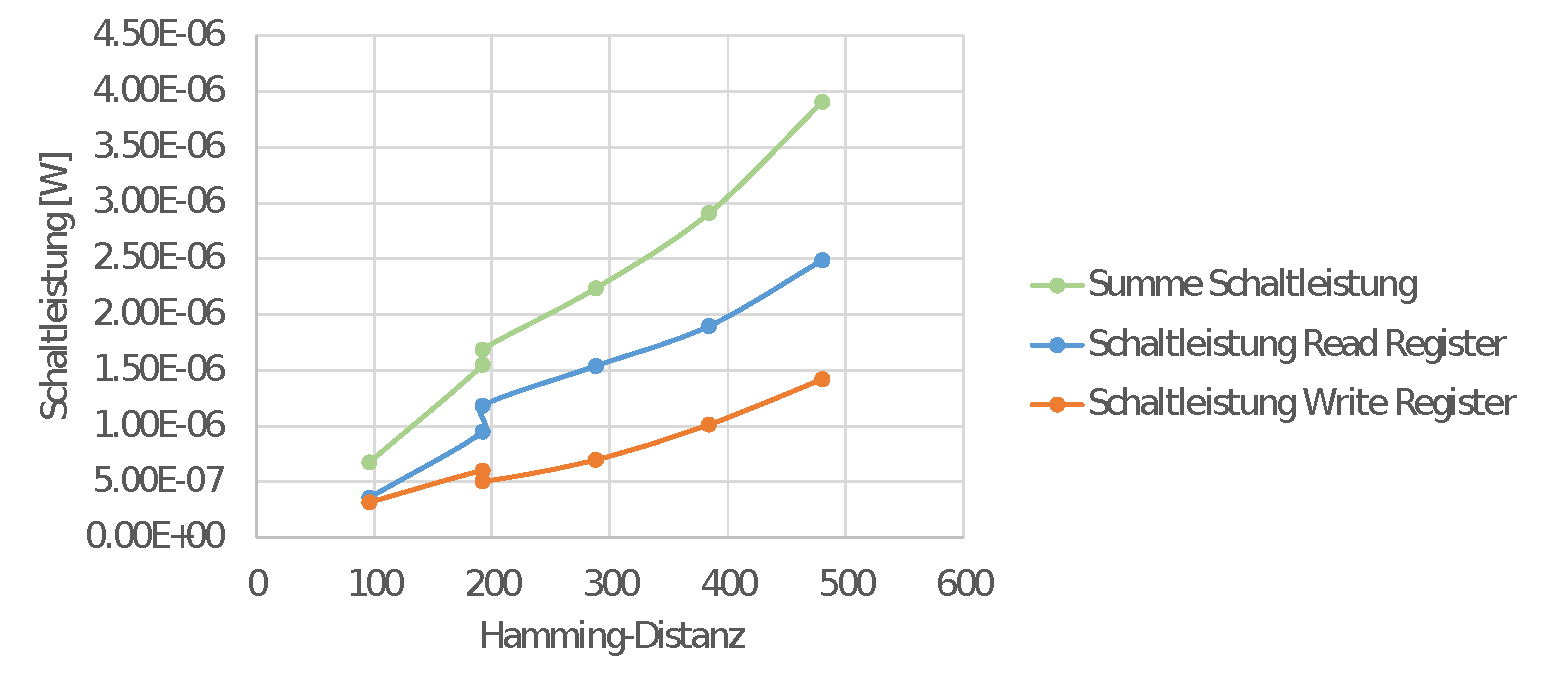
\includegraphics[width=\textwidth]{fig/source_target_power.pdf}
	\caption{Schaltleistung Read+Write Register}
	\label{fig:source_target_power}
\end{figure}

Außerdem zeigt Abbildung \ref{fig:total_power_source_target} die Gesamtleistung des Prozessors über der Hamming-Distanz. Auch hier ist eine deutliche Verbesserung erkennbar, welche sich ebenfalls linear zur Hamming-Distanz verhält.

\begin{figure}[H]
	\centering
	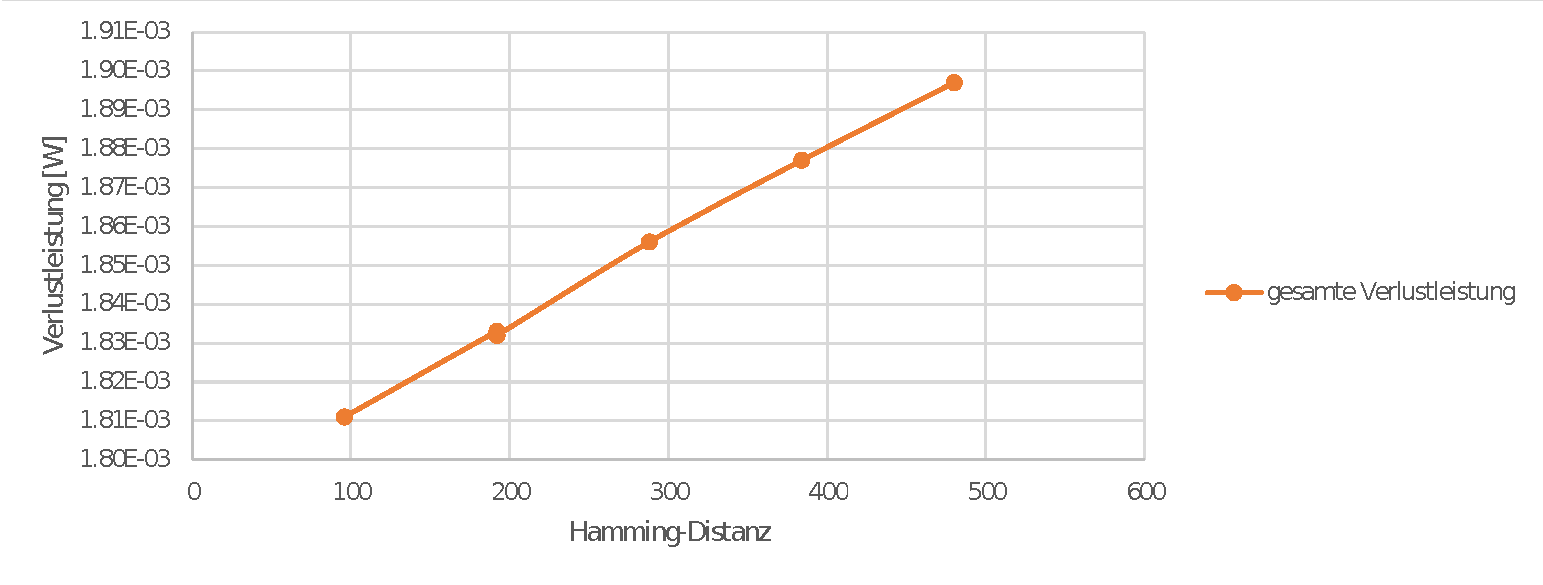
\includegraphics[width=\textwidth]{fig/total_power_source_target.pdf}
	\caption{gesamte Verlustleistung des Prozessors}
	\label{fig:total_power_source_target}
\end{figure}

Um nun ebenfalls den Einfluss der Daten auf die Verlustleistung zu ermitteln, wurden vorerst alle Register mit zufälligen Zahlen initialisiert und im Anschluss die oben beschriebenen Funktionen abgearbeitet. Diese Änderung verursacht einen Anstieg der Verlustleistung, jedoch ist zu untersuchen, ob dennoch eine Einsparung durch die Adressierung feststellbar ist. Hierzu wurden die Testfälle mehrere Male durchlaufen, so dass die Werte aussagekräftig sind. Das untenstehende Schaubild \ref{fig:random_data_total_power} zeigt die Verläufe des Testfalls der mit Null initialisierten Register in rot und mit Zufallszahlen befüllten Register in blau. Die Punktewolken verdeutlichen eine Abhängigkeit der Daten, dennoch ist ein linearer Anstieg der Verlustleistung mit der Hamming-Distanz zu erkennen. Die Linearität ist ebenfalls in der mit Null initialisierten Variante zu erkennen.

\begin{figure}[H]
	\centering
	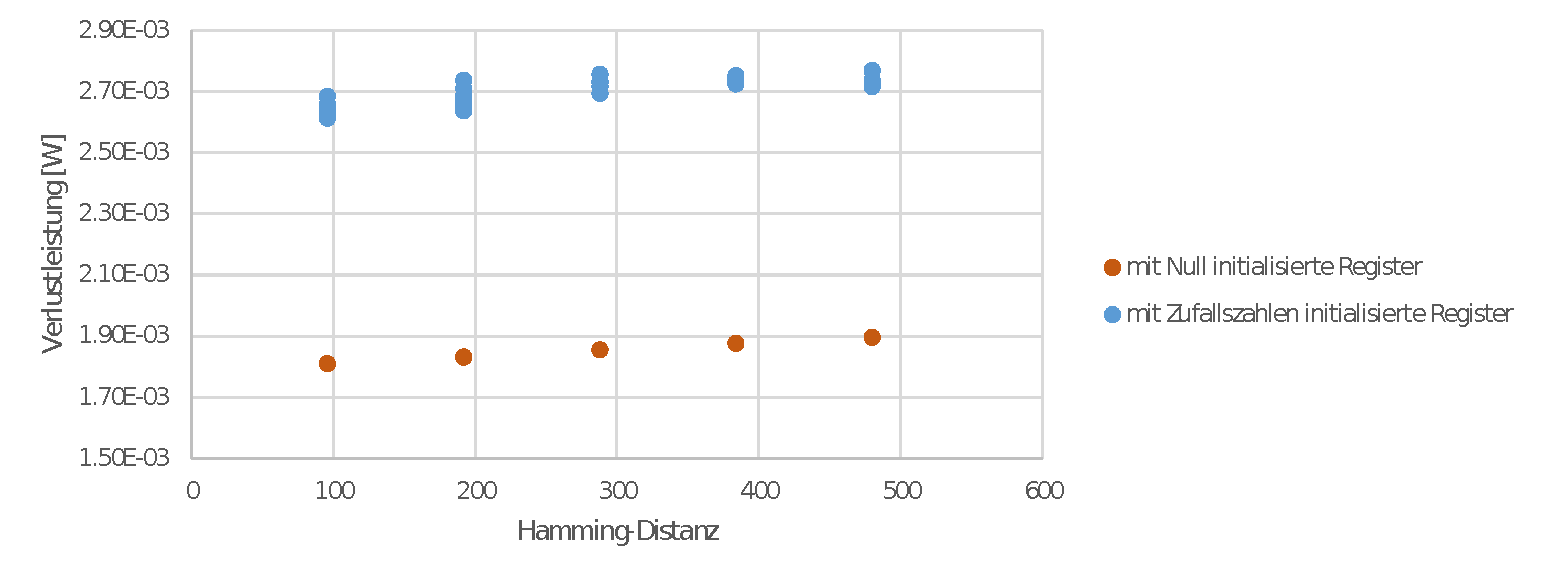
\includegraphics[width=\textwidth]{fig/random_data_total_power.pdf}
	\caption{Einfluss der Daten auf die gesamte Verlustleistung}
	\label{fig:random_data_total_power}
\end{figure}


\subsection{Heuristik}
\label{chap:eval_heuristik}
Da nun die Abhängigkeit der Register-Adressierung zu der Verlustleistung gezeigt wurde, kann dieser Ansatz durch den Einsatz von virtuellen Registern ausgenutzt werden, um eine verbesserte Heuristik zu implementieren. Hierzu werden wie in Kapitel \ref{cap:empirischeTests} Assemblerprogramme entworfen, welche manuell geschedult sind und die die Register mit Null initialisieren. Der Unterschied zu den empirischen Testprogrammen liegt darin, dass nun ebenfalls virtuelle Register verwendet werden.
Dies hat zur Folge, dass die Register-Allokation eine geeignete Zuweisung finden muss und somit die Schaltaktivität der Adresse minimieren kann. Das Testprogramm belegt vorerst durch physikalische Adressierung eine gewisse Anzahl an Registern vor und blockiert diese somit für die Verwendung von virtuellen Register (siehe Abbildung \ref{fig:heuristik_eval} - blau hinterlegte Felder).
Nachdem die Register-Files vorbelegt wurden, wird mit der Zuweisung von virtuellen Registern begonnen. Ab diesem Punkt ergeben sich Veränderungen in der Register-Allokation. Je nach gewähltem Verfahren, wird nach den optimalen physikalischen Registern mit unterschiedlichen Algorithmen gesucht. 

\begin{figure}[H] 
	\centering
	\includesvg[width=\textwidth]{heuristik_eval}
	\caption{Heuristik Evaluation}
	\label{fig:heuristik_eval}
\end{figure}
Das Schaubild \ref{fig:heuristik_eval} zeigt den Vergleich von alter zu neuer Heuristik anhand eines der implementierten Testprogramme. Die blockierten Register-Adressen sind blau hinterlegt, die von den Algorithmen ausgewählten Register-Adressen sind rot gekennzeichnet. Durch die beiden unterschiedlichen Verfahren ergibt sich ein Unterschied von 43 Schaltvorgängen in den Adress-Leitungen. Damit dieser in der Verlustleistung deutlicher zu erkennen ist, wird die Zuweisung der virtuellen Register 20 mal wiederholt. Dadurch ergibt sich eine Differenz der Hamming-Distanzen von 556. Dies ist kein Vielfaches von 43, da durch das wiederholte Ausführen der Allokation die Zuweisung mit unterschiedlichen Adressen gestartet wird.
Damit der Zusammenhang von Verlustleistung zu Schaltaktivität zu erkennen ist, wurden sechs solcher Testfälle mit unterschiedlichen Hamming-Distanzen entwickelt. Hierbei variieren die Distanzen im Bereich zwischen 1173 und 2046 für die alte Heuristik. Diese werden von der neuen Heuristik auf einen Hamming-Distanz-Bereich von 794 bis 1165 optimiert.
Die Abbildung \ref{fig:schaltleistung_heuristic}. zeigt den Verlauf der Schaltleistung an den Adressports gegenüber der Hamming-Distanz. Es ist auch hier ein linearer Verlauf der Leistung zu erkennen. Die Verschlechterung der Schaltleistung trotz höherer Hamming-Distanz lässt sich mit unterschiedlichen Lastkapazitäten begründen. Durch eine Berücksichtigung dieser, könnte die Heuristik die Verlustleistung noch besser modellieren. 
\begin{figure}[H]
	\centering
	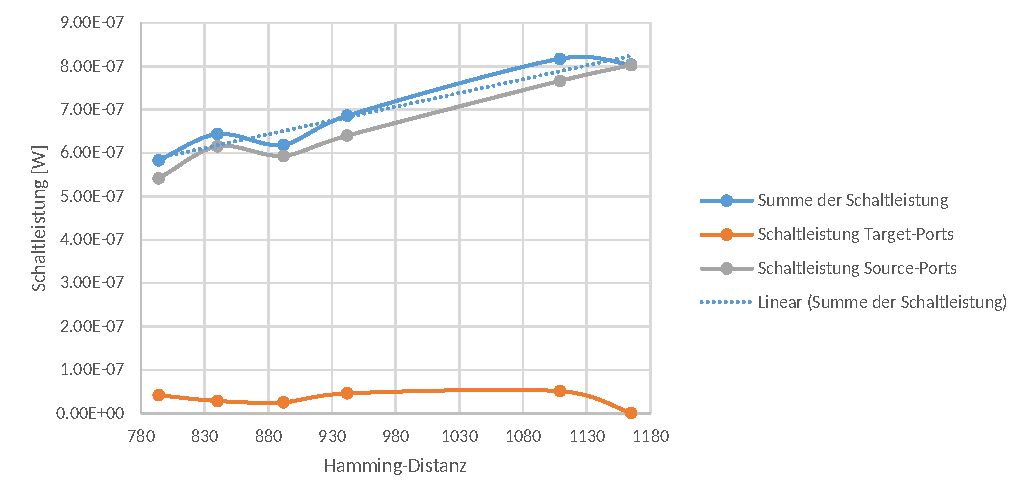
\includegraphics[width=\textwidth]{fig/schaltleistung_heuristic.pdf}
	\caption{Schaltleistung Target- und Source-Adressports}
	\label{fig:schaltleistung_heuristic}
\end{figure}

Nach der Betrachtung der Schaltleistung für die neue Heuristik zeigt Schaubild \ref{fig:heuristic_schaltleistung_alt_neu}. den Verlauf der Schaltleistungen an den Register-Ports gegenüber der Hamming-Distanz. 

\begin{figure}[H]
	\centering
	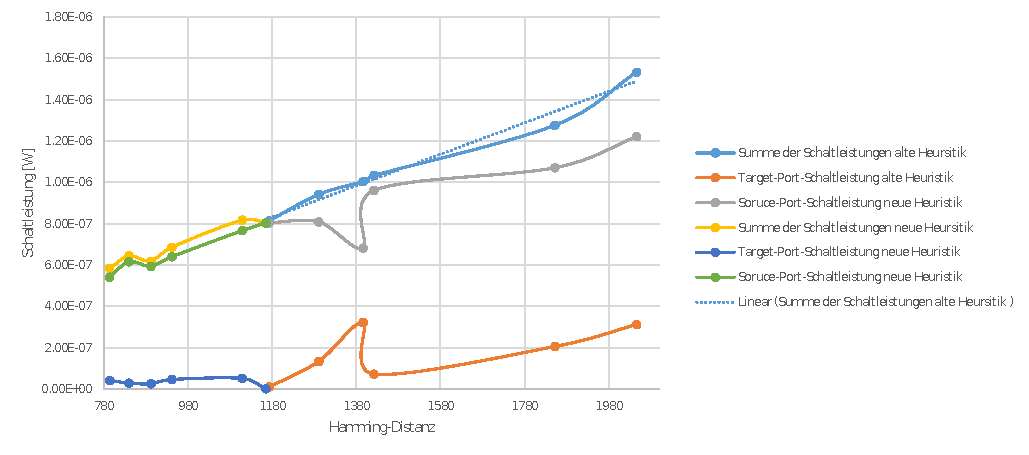
\includegraphics[width=\textwidth]{fig/heuristik_schaltleistung_alt_neu.pdf}
	\caption{Vergleich der Schaltleistungen von Target und Source-Ports}
	\label{fig:heuristic_schaltleistung_alt_neu}
\end{figure}

Dabei ist zu erkennen, dass die neu implementierte Heuristik eine deutlich bessere Lösung findet. Im Schaubild sind die Daten nach ihrer Hamming-Distanz sortiert. Demnach kann kein Vergleich der einzelnen Datenpunkte zwischen den beiden Heuristiken gezogen werden. 
Die Evaluation der Heuristik zeigt, dass für die entwickelten synthetischen Testfälle durch die neue Heuristik eine durchschnittliche Verbesserung der Schaltleistung der Adressports von 37,40\% erzielt werden kann.\\
Die Tabelle \ref{fig:compare_power_heuristic}. zeigt die Optimierung der Verlustleistung eines Testfalls, dabei sind die einzelnen Module des Prozessors gegenüber der alten Heuristik aufgeschlüsselt. Alle Werte sind in Prozent angegeben und beziehen sich auf die Gesamtleistungen der Spalten. Auch hier ist zu erkennen, dass deutliche Einsparungen in den Register-Files generiert werden konnten. Dabei wurde die Schaltleistung im Register-File gegenüber der alten Heuristik um 8,53\% verbessert. Die gesamte Verlustleistung wurde um 2,56\% optimiert. 

\begin{figure}[H]
	\centering
	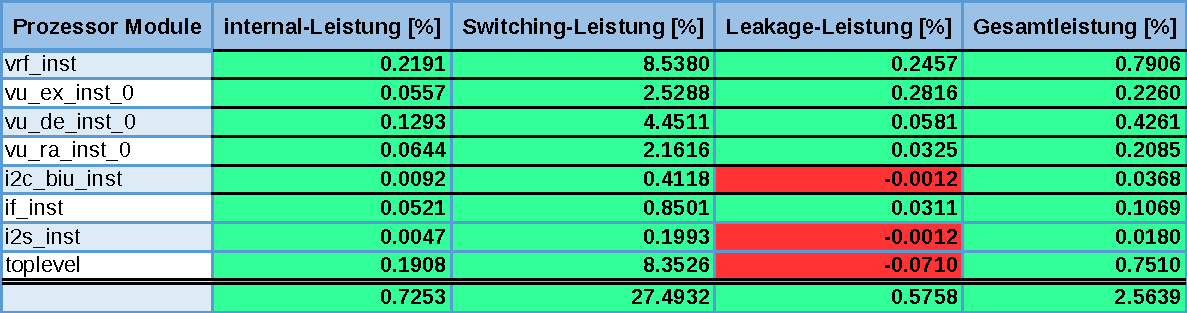
\includegraphics[width=\textwidth]{fig/compare_power_heuristic.pdf}
	\caption{Prozentuale Verbesserung der Verlustleistung - alte zu neue Heuristik}
	\label{fig:compare_power_heuristic}
\end{figure}


\subsection{Genetischer Algorithmus}
Da die Heuristik, wie bereits in Kapitel \ref{sec:genetischerAlgorithmus} erwähnt, nur die Target-Register auf Schaltaktivität minimiert, wird nun die Verbesserung der Verlustleistung durch zusätzliches Optimieren der Source-Register untersucht.
Bei der Evaluation wurde ein genetischer Algorithmus verwendet, der mit einer Heuristik eine Startpopulation berechnet, um eine schnelle Konvergenz gegen ein Minimum zu garantieren. Außerdem wird die Mutationswahrscheinlichkeit dynamisch angepasst. Als Fitness-Funktion wird die Multiplikation aus Hamming-Distanz und Lastkapazität gewählt. 
Um den Optimierungsgrad gegenüber der alten und neuen Heuristik vergleichen zu können, wurde der genetische Algorithmus mit den selben synthetischen Testprogrammen wie in Kapitel \ref{chap:eval_heuristik} getestet.
Da der genetische Algorithmus zufallsgesteuert ist, variieren die Ergebnisse stark. Um dennoch eine Aussage über die Verbesserung gegenüber der Heuristik treffen zu können, wurden die Testfälle mehrmals ausgeführt. Das Schaubild \ref{fig:schaltleistung_genetic_heuristik} zeigt, wie stark die Ergebnisse der gesamten Schaltleistung untereinander variieren. Dabei ist zu erkennen, dass der genetische Algorithmus in den meisten Fällen eine Verbesserung gegenüber der neuen Heuristik findet. In Testfall vier wurde vom genetischen Algorithmus keine Verbesserung gefunden, da die Heuristik für dieses Szenario bereits eine Lösung gefunden hat, die der Algorithmus in seiner Laufzeit nicht weiter minimieren konnte.  
\begin{figure}[H]
	\centering
	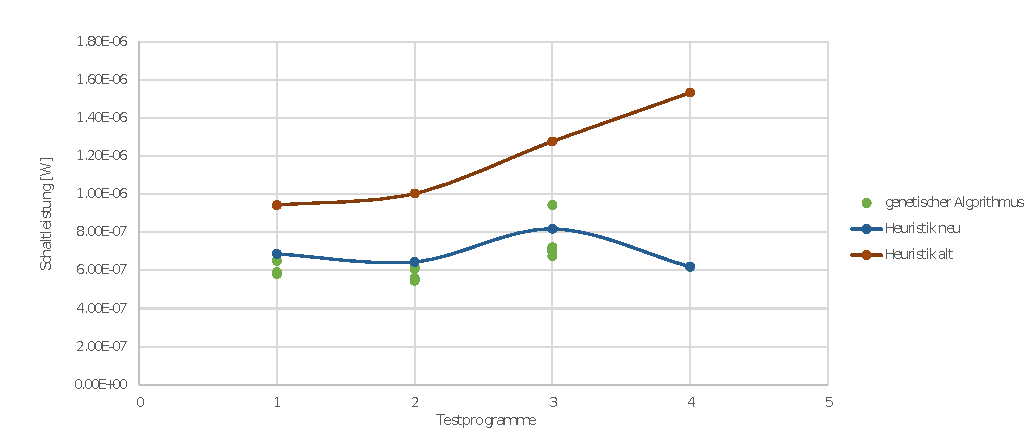
\includegraphics[width=\textwidth]{fig/schaltleistung_genetic_heuristik.pdf}
	\caption{Vergleich der Schaltleistungen für Heuristik und genetischer Algorithmus}
	\label{fig:schaltleistung_genetic_heuristik}
\end{figure}
Die durchschnittliche Verbesserung der Schaltleistung gegenüber der neuen Heuristik beträgt 7,83\% und 41,57\% im Vergleich zur alten Heuristik. Der genetische Algorithmus konnte im besten Fall eine Verbesserung von 17,38\% zur neuen Heuristik und 59,70\% zur alte Heuristik erreichen.\\
Das Schaubild \ref{fig:eval_genetic_total_power} veranschaulicht die Ergebnisse der Gesamtleistung des Prozessors. Dabei ist zu erkennen, dass die Leistung minimiert wurde, der genetische Algorithmus jedoch die Gesamtleistung nicht verbessern konnte. Die neue Heuristik konnte im Durchschnitt eine Verbesserung der Verlustleistung von 1,82\% erreichen. Im Gegensatz hierzu konnte der genetische Algorithmus die Verlustleistung nur auf 1,62\% optimieren. Dies impliziert, dass die Gesamtleistung noch von anderen Parametern abhängt und die Fitness-Funktion an diese angepasst werden muss.

\begin{figure}[H]
	\centering
	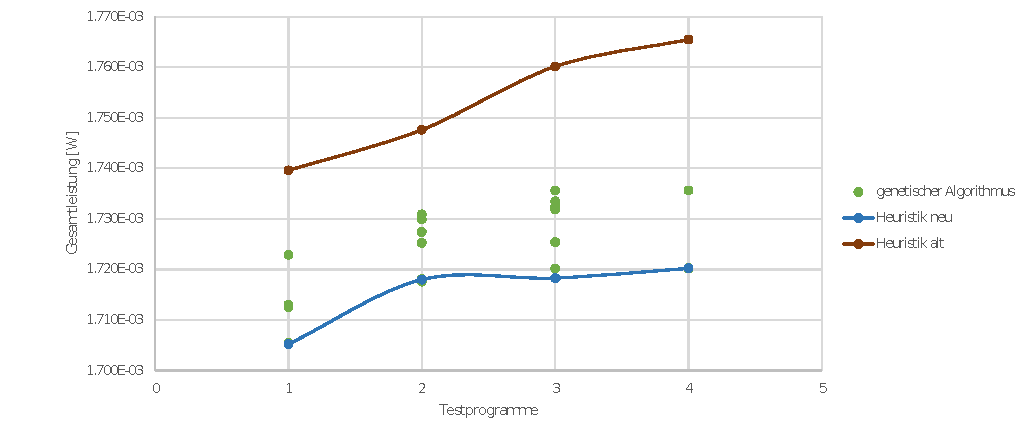
\includegraphics[width=\textwidth]{fig/gesamtleistung_genetik_heuristik.pdf}
	\caption{Gesamtverlustleistung genetischer Algorithmus vs. Heuristik}
	\label{fig:eval_genetic_total_power}
\end{figure}

Die komplette Einsparung fällt relativ gering aus, jedoch ist hervorzuheben, dass diese Optimierung ohne Veränderung der Hardware erzielt werden kann und keine Einbußen in Performance sowie Chipfläche generiert werden.
%Im unten stehenden Schaubild XXX wird der Mittelwert der Testfälle gegenüber der alten Heuristik veranschaulicht. 
%
%Mittelwert genetischer Algo gegenüber alter heuristik

Auch in Tabelle \ref{fig:power_percent_genetic} zeigt ein prozentualer Vergleich der Verlustleistungen des kompletten Prozessors eine Verbesserung der Schaltleistung in den Register-Files. In diesem Fall wird die beste Lösung des genetischen Algorithmus mit der alten Heuristik verglichen. Die Tabelle zeigt eine Verbesserung der Schaltleistung des gesamten Prozessors um 28,31\% und eine Einsparung der Gesamtleistung um 2,56\%. Die Verlustleistung, die durch die Leakage-Ströme verursacht wird, ist um zwei bzw. drei Zehnerpotenzen kleiner als die Verlustleistungen die durch die Schaltvorgänge hervorgerufen werden. Aus diesem Grund werden diese vernachlässigt. 
Die prozentuale Veränderung der Internal-Leistung liegt im niedrigen Prozentbereich und wird ebenfalls nicht weiter berücksichtigt. 

\begin{figure}[H]
	\centering
	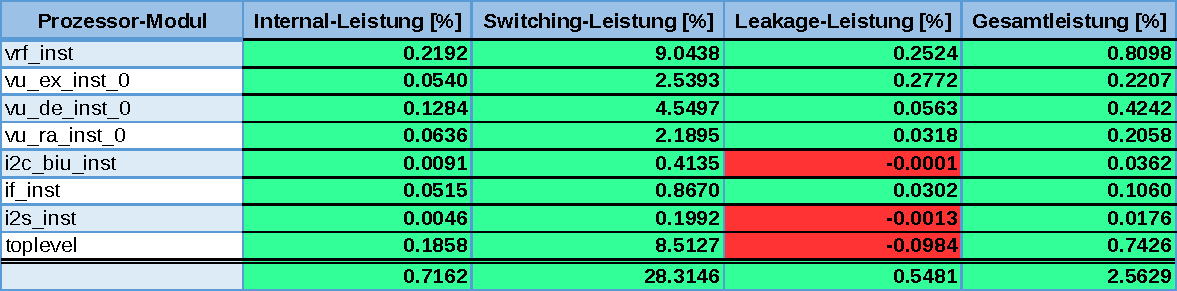
\includegraphics[width=\textwidth]{fig/power_percent_genetic.pdf}
	\caption{Prozentuale Verbesserung der Verlustleistung}
	\label{fig:power_percent_genetic}
\end{figure}

Die Schaubilder \ref{fig:totalpower_old}, \ref{fig:totalpower_new} sowie \ref{fig:totalpower_genetic} zeigen den Verlauf der Gesamtleistung des Prozessors gegenüber der Hamming-Distanz.

\begin{figure}[H]
	\centering
	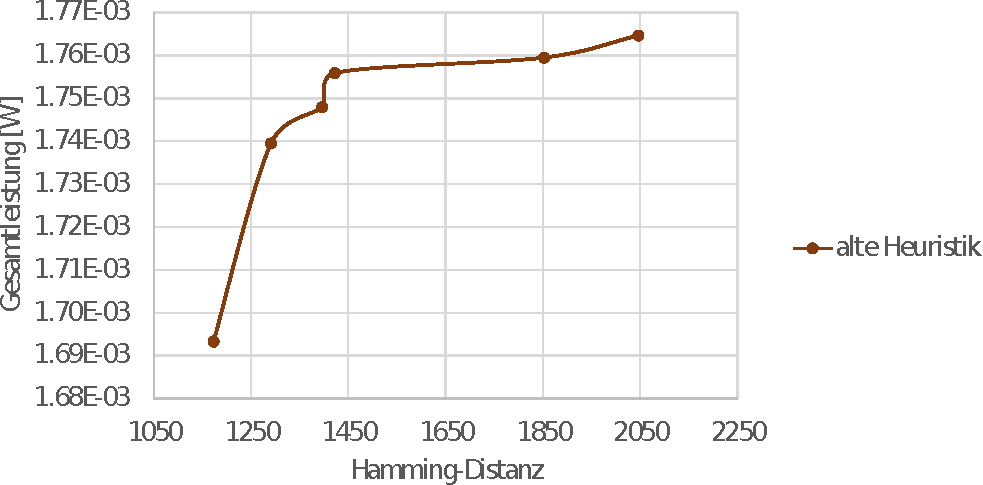
\includegraphics[width=\textwidth]{fig/totalpower_old.pdf}
	\caption{Verlauf der Gesamtleistung alte Heuristik }
	\label{fig:totalpower_old}
\end{figure}

\begin{figure}[H]
	\centering
	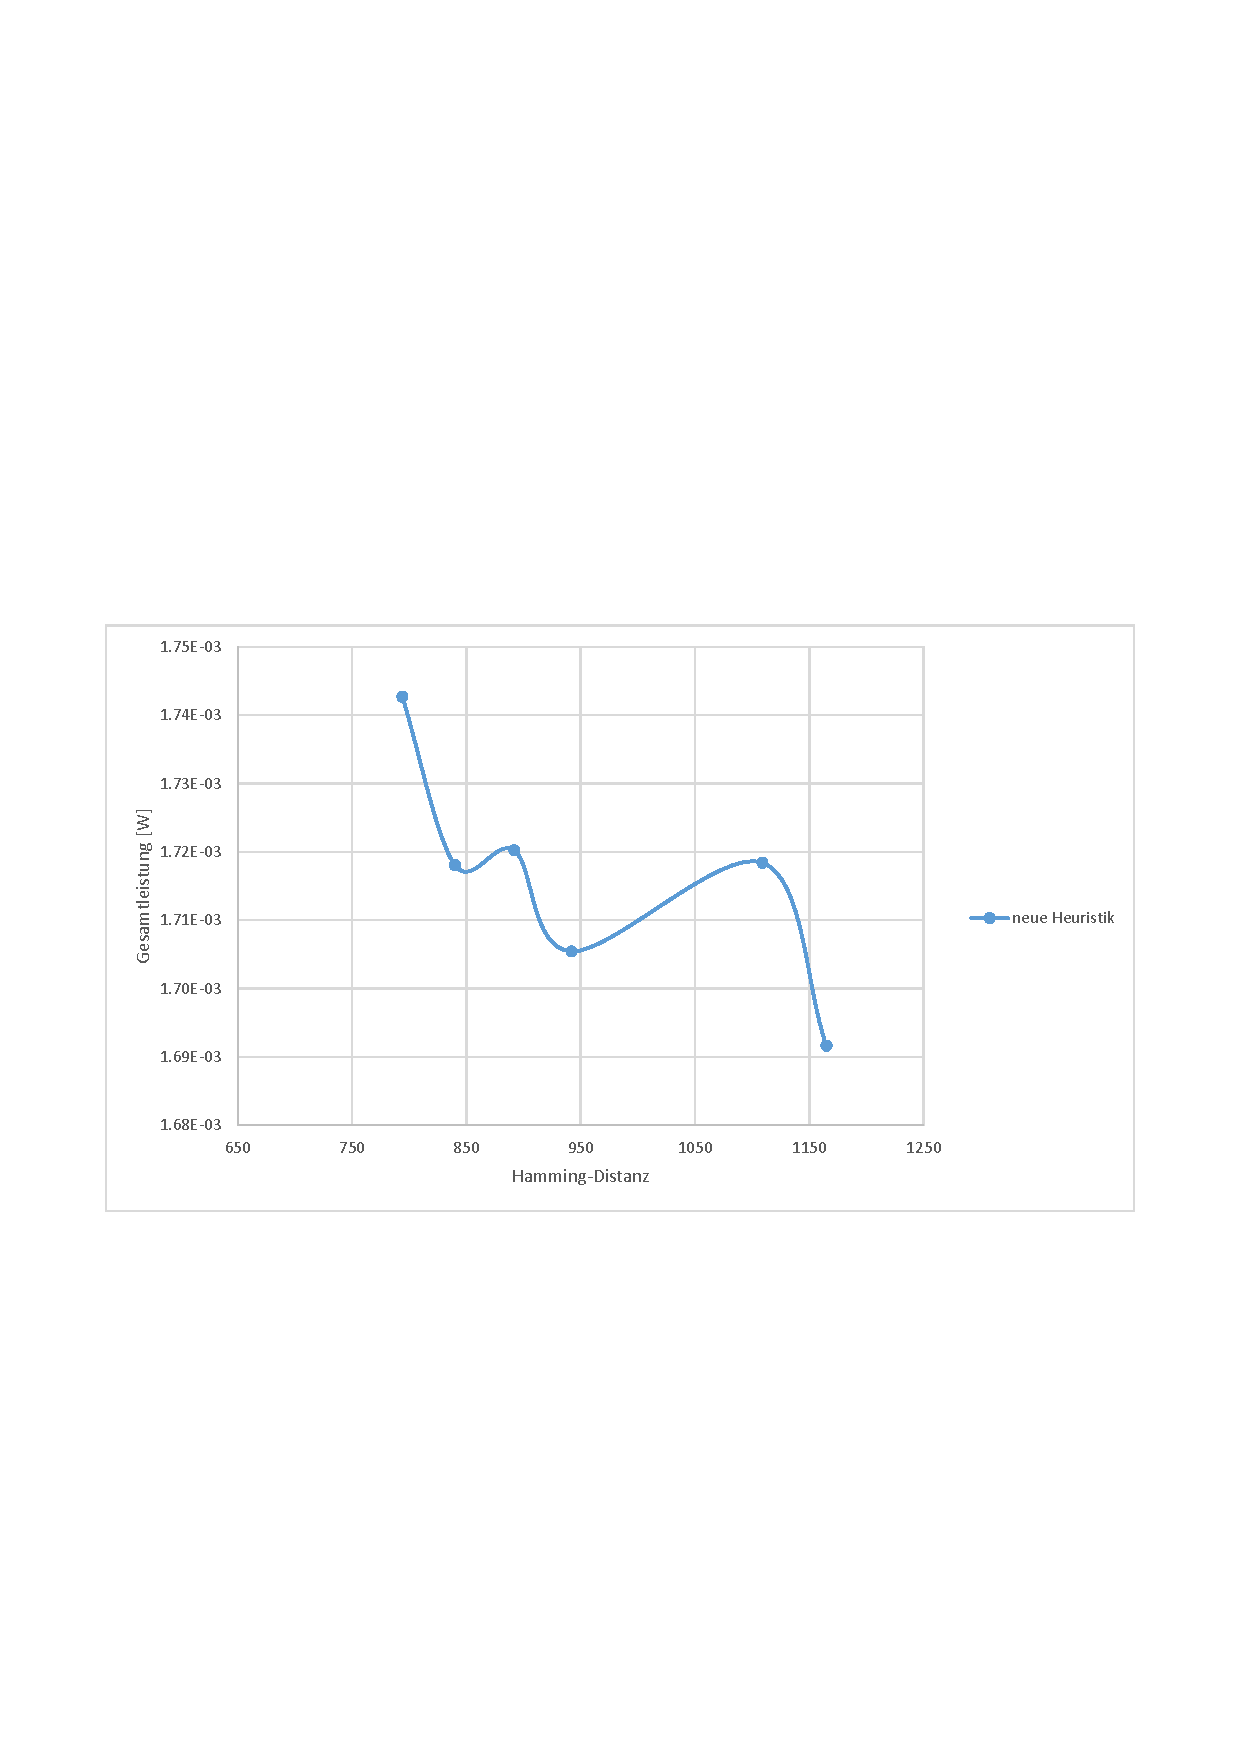
\includegraphics[width=\textwidth]{fig/totalpower_new.pdf}
	\caption{Verlauf der Gesamtleistung neue Heuristik}
	\label{fig:totalpower_new}
\end{figure}

\begin{figure}[H]
	\centering
	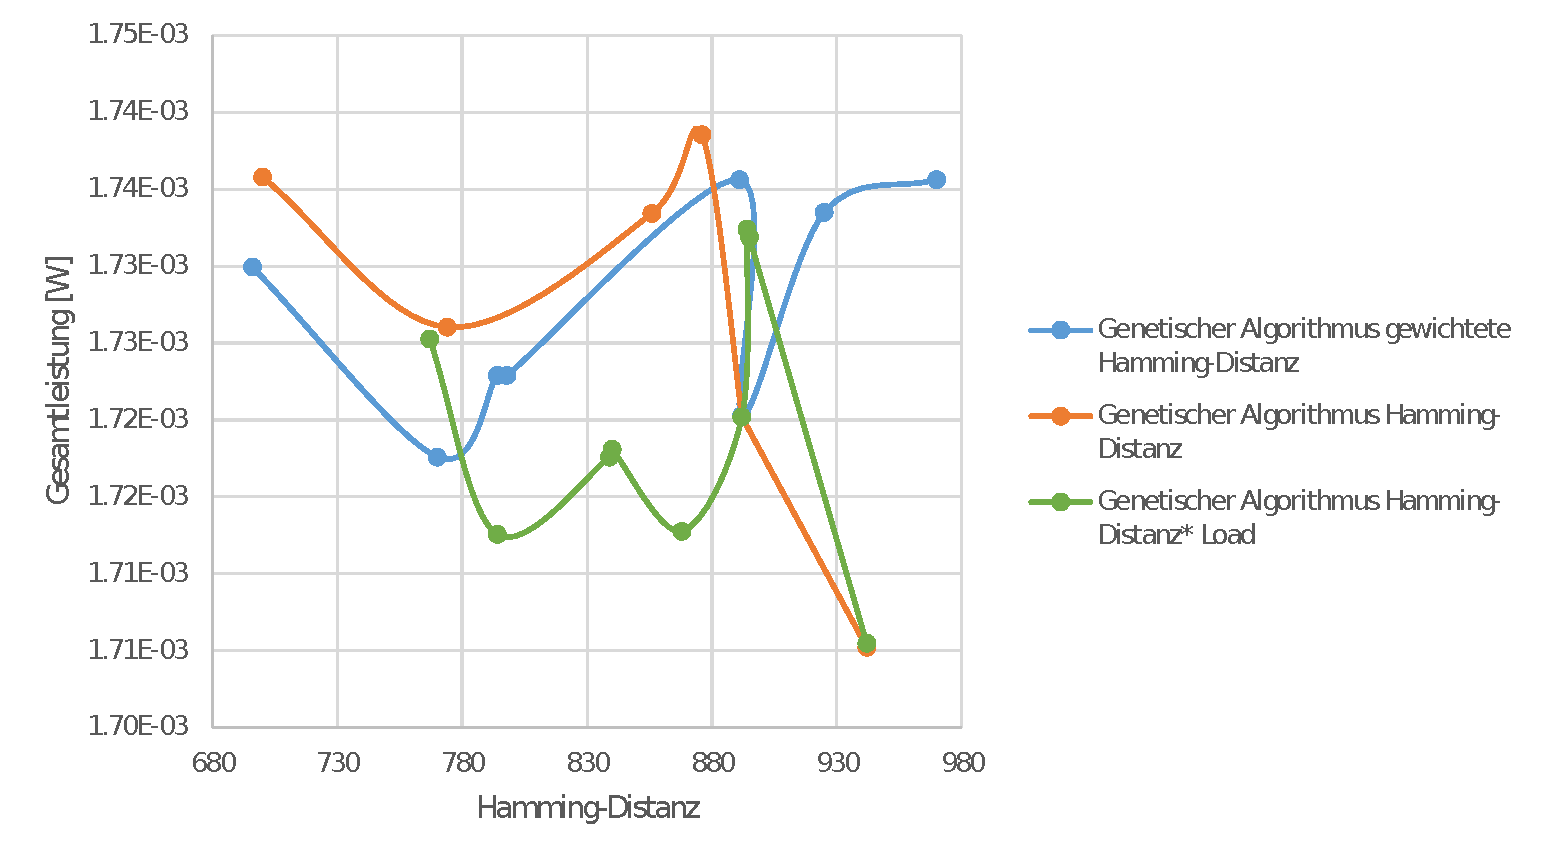
\includegraphics[width=\textwidth]{fig/totalpower_genetic.pdf}
	\caption{Verlauf der Gesamtleistung genetischer Algorithmus}
	\label{fig:totalpower_genetic}
\end{figure}

Bei der Gesamtleistung für die neue Heuristik ist auffällig, dass die Leistung mit steigender Hamming-Distanz fällt. Das selbe Verhalten ist für den genetischen Algorithmus erkennbar. Im Gegensatz hierzu steigt die Leistung der alte Heuristik mit der Hamming-Distanz an. Dieses Phänomen muss näher untersucht werden, was jedoch den Umfang dieser Arbeit übersteigt.

\section{Hörgerätealgorithmen}
\label{sec:testprogamme}
Um den implementierten Code zu testen und eine reale Einsparung der Verlustleistungsreduktion zu ermitteln, wurden die folgenden Hörgerätealgorithmen verwendet. Dabei handelt es sich um Programme, die eine häufig Anwendung in Hörgerät-Prozessoren finden.

\subsection{Emulated Floating Point}
\label{chap:emulated_floating_point}
Da der verwendete Prozessor keine Gleitkommavariablen unterstützt, besteht eine softwarebasierte Methode der diese emuliert. Dabei wird eine Gleitkommazahl als zwei Subworte deklariert, zum einen der Signifikant $T$ und zum anderen der Exponent $E$. Mit Hilfe dieser kann eine Gleitkommazahl $f$ nach Formel \ref{eq:emulated_floating_point} berechnet werden.
\begin{equation}
f = T *2^E
\label{eq:emulated_floating_point}
\end{equation}
Beide Variablen $T$ und $E$ können als Subwort im Register gespeichert werden. Dabei können diese an einer beliebigen Adresse des Registers stehen. Aus diesem Grund werden hierfür zwei virtuelle Register verwendet. Diese Emulation ist besonders für SIMD-Architekturen geeignet, bei denen eine Gleitkommaberechnung ohne Aufschlüsseln der Variablen errechnet werden kann. Dadurch ist diese Art von Gleitkommaberechnung äußerst performant.
Wenn nun ein Algorithmus mit Gleitkommazahlen rechnet, werden viele temporäre Zwischenwerte berechnet, was den Algorithmus prädestiniert für eine Adressoptimierung macht. Aus diesem Grund wurden  Algorithmen verwendet, die mit diesen arbeiten. \cite{gerlach2016efficient}

\subsection{Filter und FFT mit Emulated Floating Point}
Im Folgenden wird die Verlustleistung der beiden Algorithmen zur \glqq Fast-Fourier-Transformation\grqq{ }(FFT) und zu einem Frequenzfilter analysiert. Die beiden Abbildungen XXX zeigen die Einsparungen die durch die neue Heursistik und den genetischen Algorithmus erreicht wurden.

Abbildungen FFT und Filter emulated floating point

Im Fall der FFT ist eine Optimierung der Verlustleistung um XXX\% erreichbar. Dabei ist anzumerken, dass die Problemstellung der FFT mit nahe zu 8000 Instruktionen groß ausfällt und der genetische Algorithmus nur geringe Verbesserungen finden konnte. Durch ein längere Testdauer sollte es dem genetischen Algorithmus jedoch möglich sein, weitere Verbesserungen zu finden.

%\subsection{Filter emulated floating Point} Der Filter mit Gleitkommazahl-Berechnung konnte hingegen eine Einsprung von XXX\% erzielen.



%\subsection{Beamforming}
%Der Beamforming-Algorithmus wird eingesetzt um eine Positionsbestimmung von Schallwellen im Raum durchzuführen und somit eine Ein- bzw Ausblendung von verschiedenen Geräuschen zu gewährleisten und so das Hörerlebnis zu steigern. 

 


\section{Einfluss der Register-Daten auf die Verlustleistung}
In Kapitel \ref{cap:empirischeTests} wurde bereits der Einfluss der Daten auf die Verlustleistung ermittelt. Da sich nun jedoch eine Verschlechterung der Register-File-Leistung bei besserer Adressierung in den realen Testfällen ergibt, wurde die Datenabhängigkeit nochmals überprüft. Dabei ergab sich, dass auf Grund des Verhaltens des Adress-Decoders eine Veränderung der Daten verursacht wird. Da die Adressen über einen Adress-Decoder decodiert werden müssen und dieser nicht direkt alle Bits auf einmal umschalten kann, liegen über einen kurzen Zeitraum Daten aus anderen Adressen an den Daten-Leitungen an. Dies verursacht dort Schaltleistungen, welche die Verbesserung durch die Adressierung aufheben.
%Um dieses Verhalten und die Funktion des Decoders besser nachzuvollziehen wurden nun weitere Testfälle generiert. Diese befüllen wie in Kapitel \ref{cap:empirischeTests} alle Register mit zufälligen Daten. Der unterschied liegt jedoch darin, dass die Instruktionen in allen Testfällen mit den selben Zufallsdaten arbeiten, so dass immer die selben Daten in die entsprechenden Register geschrieben werden.
%
%Hierbei war zu erkennen, 

\section{Einfluss der Lastkapazität auf die Verlustleistung}
 \label{cap:lastkapa}
Wie bereits in Kapitel \ref{cap:empirischeTests} erwähnt, besteht eine Abhängigkeit zwischen Lastkapazität und Verlustleistung. Dies lässt sich auf die Formel (\ref{eq:dynVerlustleistung}) der dynamischen Verlustleistung zurückführen. Laut dieser steigt die Verlustleistung linear mit der Lastkapazität an.
Das nachfolgende Schaubild \ref{fig:read_port_mux} zeigt, wie die Daten aus den Registern an die Read-Ports angelegt werden. Hierbei ist jedes Bit der Register-Adresse für das Schalten eines Multiplexers zuständig. Besteht nun der Fall, dass ein Register mit einer Adresse von 31 ausgelesen werden soll, so müssen alle Multiplexer durchschalten. Dadurch werden die Daten des Registers an den verwendeten Register-Port weitergeleitet. Wird im Gegensatz hierzu eine niedrige Adresse, beispielsweise Null, angefragt, so muss keiner der Multiplexer schalten. Das Signal liegt direkt an dem Read-Port an. Aus diesem Grund benötigen die oberen Adressleitungen mehr Verlustleistung, da das Signal eine höhere Lastkapazität aufweist. Dies lässt sich ebenfalls in den Power-Reports nachvollziehen. Dort ist deutlich zu erkennen, dass die oberen Register-Adressen eine höhere Lastkapazität aufweisen. 
\begin{scriptsize}
	\begin{figure}[htbp] 
		\centering
		\includesvg[width=\textwidth]{Read-Port-Mux}
		\caption{Read-Port Multiplexer}
		\label{fig:read_port_mux}
	\end{figure}
\end{scriptsize}

Aus diesem Grund wurde die Fitness Funktion des genetischen Algorithmus so angepasst, dass die Lastkapazität zusätzlich berücksichtigt wird.
